% Options for packages loaded elsewhere
\PassOptionsToPackage{unicode}{hyperref}
\PassOptionsToPackage{hyphens}{url}
%
\documentclass[
]{article}
\usepackage{amsmath,amssymb}
\usepackage{iftex}
\ifPDFTeX
  \usepackage[T1]{fontenc}
  \usepackage[utf8]{inputenc}
  \usepackage{textcomp} % provide euro and other symbols
\else % if luatex or xetex
  \usepackage{unicode-math} % this also loads fontspec
  \defaultfontfeatures{Scale=MatchLowercase}
  \defaultfontfeatures[\rmfamily]{Ligatures=TeX,Scale=1}
\fi
\usepackage{lmodern}
\ifPDFTeX\else
  % xetex/luatex font selection
\fi
% Use upquote if available, for straight quotes in verbatim environments
\IfFileExists{upquote.sty}{\usepackage{upquote}}{}
\IfFileExists{microtype.sty}{% use microtype if available
  \usepackage[]{microtype}
  \UseMicrotypeSet[protrusion]{basicmath} % disable protrusion for tt fonts
}{}
\makeatletter
\@ifundefined{KOMAClassName}{% if non-KOMA class
  \IfFileExists{parskip.sty}{%
    \usepackage{parskip}
  }{% else
    \setlength{\parindent}{0pt}
    \setlength{\parskip}{6pt plus 2pt minus 1pt}}
}{% if KOMA class
  \KOMAoptions{parskip=half}}
\makeatother
\usepackage{xcolor}
\usepackage[margin=1in]{geometry}
\usepackage{color}
\usepackage{fancyvrb}
\newcommand{\VerbBar}{|}
\newcommand{\VERB}{\Verb[commandchars=\\\{\}]}
\DefineVerbatimEnvironment{Highlighting}{Verbatim}{commandchars=\\\{\}}
% Add ',fontsize=\small' for more characters per line
\usepackage{framed}
\definecolor{shadecolor}{RGB}{248,248,248}
\newenvironment{Shaded}{\begin{snugshade}}{\end{snugshade}}
\newcommand{\AlertTok}[1]{\textcolor[rgb]{0.94,0.16,0.16}{#1}}
\newcommand{\AnnotationTok}[1]{\textcolor[rgb]{0.56,0.35,0.01}{\textbf{\textit{#1}}}}
\newcommand{\AttributeTok}[1]{\textcolor[rgb]{0.13,0.29,0.53}{#1}}
\newcommand{\BaseNTok}[1]{\textcolor[rgb]{0.00,0.00,0.81}{#1}}
\newcommand{\BuiltInTok}[1]{#1}
\newcommand{\CharTok}[1]{\textcolor[rgb]{0.31,0.60,0.02}{#1}}
\newcommand{\CommentTok}[1]{\textcolor[rgb]{0.56,0.35,0.01}{\textit{#1}}}
\newcommand{\CommentVarTok}[1]{\textcolor[rgb]{0.56,0.35,0.01}{\textbf{\textit{#1}}}}
\newcommand{\ConstantTok}[1]{\textcolor[rgb]{0.56,0.35,0.01}{#1}}
\newcommand{\ControlFlowTok}[1]{\textcolor[rgb]{0.13,0.29,0.53}{\textbf{#1}}}
\newcommand{\DataTypeTok}[1]{\textcolor[rgb]{0.13,0.29,0.53}{#1}}
\newcommand{\DecValTok}[1]{\textcolor[rgb]{0.00,0.00,0.81}{#1}}
\newcommand{\DocumentationTok}[1]{\textcolor[rgb]{0.56,0.35,0.01}{\textbf{\textit{#1}}}}
\newcommand{\ErrorTok}[1]{\textcolor[rgb]{0.64,0.00,0.00}{\textbf{#1}}}
\newcommand{\ExtensionTok}[1]{#1}
\newcommand{\FloatTok}[1]{\textcolor[rgb]{0.00,0.00,0.81}{#1}}
\newcommand{\FunctionTok}[1]{\textcolor[rgb]{0.13,0.29,0.53}{\textbf{#1}}}
\newcommand{\ImportTok}[1]{#1}
\newcommand{\InformationTok}[1]{\textcolor[rgb]{0.56,0.35,0.01}{\textbf{\textit{#1}}}}
\newcommand{\KeywordTok}[1]{\textcolor[rgb]{0.13,0.29,0.53}{\textbf{#1}}}
\newcommand{\NormalTok}[1]{#1}
\newcommand{\OperatorTok}[1]{\textcolor[rgb]{0.81,0.36,0.00}{\textbf{#1}}}
\newcommand{\OtherTok}[1]{\textcolor[rgb]{0.56,0.35,0.01}{#1}}
\newcommand{\PreprocessorTok}[1]{\textcolor[rgb]{0.56,0.35,0.01}{\textit{#1}}}
\newcommand{\RegionMarkerTok}[1]{#1}
\newcommand{\SpecialCharTok}[1]{\textcolor[rgb]{0.81,0.36,0.00}{\textbf{#1}}}
\newcommand{\SpecialStringTok}[1]{\textcolor[rgb]{0.31,0.60,0.02}{#1}}
\newcommand{\StringTok}[1]{\textcolor[rgb]{0.31,0.60,0.02}{#1}}
\newcommand{\VariableTok}[1]{\textcolor[rgb]{0.00,0.00,0.00}{#1}}
\newcommand{\VerbatimStringTok}[1]{\textcolor[rgb]{0.31,0.60,0.02}{#1}}
\newcommand{\WarningTok}[1]{\textcolor[rgb]{0.56,0.35,0.01}{\textbf{\textit{#1}}}}
\usepackage{graphicx}
\makeatletter
\def\maxwidth{\ifdim\Gin@nat@width>\linewidth\linewidth\else\Gin@nat@width\fi}
\def\maxheight{\ifdim\Gin@nat@height>\textheight\textheight\else\Gin@nat@height\fi}
\makeatother
% Scale images if necessary, so that they will not overflow the page
% margins by default, and it is still possible to overwrite the defaults
% using explicit options in \includegraphics[width, height, ...]{}
\setkeys{Gin}{width=\maxwidth,height=\maxheight,keepaspectratio}
% Set default figure placement to htbp
\makeatletter
\def\fps@figure{htbp}
\makeatother
\setlength{\emergencystretch}{3em} % prevent overfull lines
\providecommand{\tightlist}{%
  \setlength{\itemsep}{0pt}\setlength{\parskip}{0pt}}
\setcounter{secnumdepth}{-\maxdimen} % remove section numbering
\ifLuaTeX
  \usepackage{selnolig}  % disable illegal ligatures
\fi
\IfFileExists{bookmark.sty}{\usepackage{bookmark}}{\usepackage{hyperref}}
\IfFileExists{xurl.sty}{\usepackage{xurl}}{} % add URL line breaks if available
\urlstyle{same}
\hypersetup{
  hidelinks,
  pdfcreator={LaTeX via pandoc}}

\author{}
\date{\vspace{-2.5em}}

\begin{document}

\begin{Shaded}
\begin{Highlighting}[]
\CommentTok{\#install tmap to upgrade it each time when reopen the file}
\CommentTok{\#install.packages(\textquotesingle{}tmap\textquotesingle{})}
\FunctionTok{library}\NormalTok{(fs)}
\FunctionTok{library}\NormalTok{(terra)}
\end{Highlighting}
\end{Shaded}

\begin{verbatim}
## terra 1.7.55
\end{verbatim}

\begin{Shaded}
\begin{Highlighting}[]
\FunctionTok{library}\NormalTok{(tidyverse)}
\end{Highlighting}
\end{Shaded}

\begin{verbatim}
## -- Attaching packages --------------------------------------- tidyverse 1.3.0 --
\end{verbatim}

\begin{verbatim}
## v ggplot2 3.4.4     v purrr   1.0.2
## v tibble  3.2.1     v dplyr   1.1.3
## v tidyr   1.3.0     v stringr 1.5.1
## v readr   2.1.4     v forcats 1.0.0
\end{verbatim}

\begin{verbatim}
## -- Conflicts ------------------------------------------ tidyverse_conflicts() --
## x tidyr::extract() masks terra::extract()
## x dplyr::filter()  masks stats::filter()
## x dplyr::lag()     masks stats::lag()
\end{verbatim}

\begin{Shaded}
\begin{Highlighting}[]
\FunctionTok{library}\NormalTok{(tmap)}
\end{Highlighting}
\end{Shaded}

\begin{verbatim}
## Breaking News: tmap 3.x is retiring. Please test v4, e.g. with
## remotes::install_github('r-tmap/tmap')
\end{verbatim}

\begin{Shaded}
\begin{Highlighting}[]
\CommentTok{\# flist \textless{}{-} dir\_ls("data")}
\NormalTok{baulogg }\OtherTok{\textless{}{-}}\FunctionTok{rast}\NormalTok{(}\StringTok{"bau\_logg\_final.tif"}\NormalTok{) }
\NormalTok{baufire }\OtherTok{\textless{}{-}}\FunctionTok{rast}\NormalTok{(}\StringTok{"bau\_fire\_final.tif"}\NormalTok{)}
\NormalTok{fire }\OtherTok{\textless{}{-}} \FunctionTok{rast}\NormalTok{(}\StringTok{"fire.tif"}\NormalTok{)}
\NormalTok{drought }\OtherTok{\textless{}{-}} \FunctionTok{rast}\NormalTok{(}\StringTok{"drought.tif"}\NormalTok{)}
\NormalTok{edge }\OtherTok{\textless{}{-}} \FunctionTok{rast}\NormalTok{(}\StringTok{"edge.tif"}\NormalTok{)}
\NormalTok{logging }\OtherTok{\textless{}{-}} \FunctionTok{rast}\NormalTok{(}\StringTok{"logging.tif"}\NormalTok{)}
\end{Highlighting}
\end{Shaded}

\begin{Shaded}
\begin{Highlighting}[]
\CommentTok{\#tm\_shape(baulogg)+tm\_raster()+tm\_basemap()}
\FunctionTok{data}\NormalTok{(}\StringTok{"World"}\NormalTok{)}
\NormalTok{baulogg[baulogg }\SpecialCharTok{\textless{}} \DecValTok{0}\NormalTok{] }\OtherTok{\textless{}{-}} \ConstantTok{NA}
\NormalTok{logmap }\OtherTok{\textless{}{-}} \FunctionTok{tm\_shape}\NormalTok{(World,}\AttributeTok{bbox =}\NormalTok{ stars}\SpecialCharTok{::}\FunctionTok{st\_as\_stars}\NormalTok{(baulogg))}\SpecialCharTok{+}\FunctionTok{tm\_polygons}\NormalTok{() }\SpecialCharTok{+}
  \FunctionTok{tm\_shape}\NormalTok{(baulogg)}\SpecialCharTok{+}\FunctionTok{tm\_raster}\NormalTok{()}
\FunctionTok{print}\NormalTok{(logmap)}
\end{Highlighting}
\end{Shaded}

\begin{verbatim}
## stars object downsampled to 1140 by 877 cells. See tm_shape manual (argument raster.downsample)
\end{verbatim}

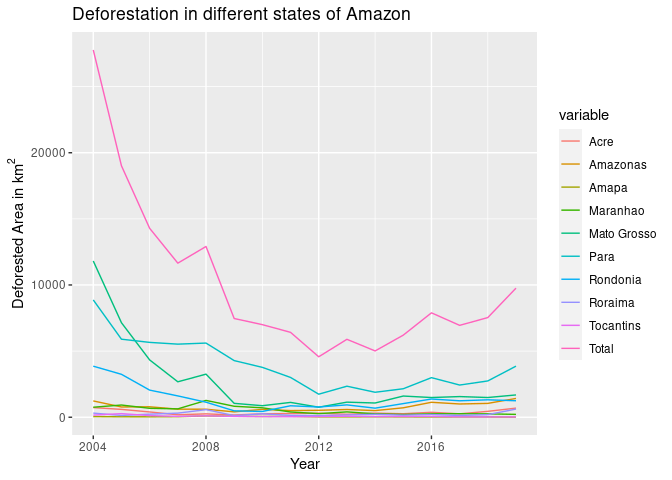
\includegraphics{Fire_files/figure-latex/unnamed-chunk-3-1.pdf}

\begin{Shaded}
\begin{Highlighting}[]
\NormalTok{baufire[baufire }\SpecialCharTok{\textless{}} \DecValTok{0}\NormalTok{] }\OtherTok{\textless{}{-}} \ConstantTok{NA}
\FunctionTok{tm\_shape}\NormalTok{(World,}\AttributeTok{bbox =}\NormalTok{ stars}\SpecialCharTok{::}\FunctionTok{st\_as\_stars}\NormalTok{(baufire))}\SpecialCharTok{+}\FunctionTok{tm\_polygons}\NormalTok{() }\SpecialCharTok{+}
  \FunctionTok{tm\_shape}\NormalTok{(baufire)}\SpecialCharTok{+}\FunctionTok{tm\_raster}\NormalTok{()}
\end{Highlighting}
\end{Shaded}

\begin{verbatim}
## stars object downsampled to 1140 by 877 cells. See tm_shape manual (argument raster.downsample)
\end{verbatim}

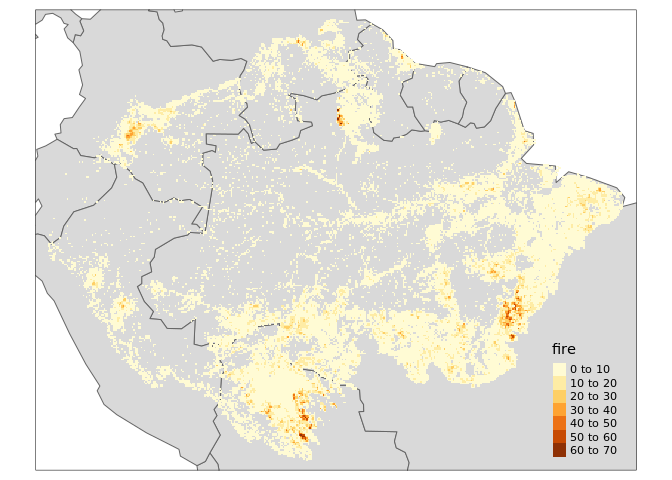
\includegraphics{Fire_files/figure-latex/unnamed-chunk-4-1.pdf}

\begin{Shaded}
\begin{Highlighting}[]
\NormalTok{fire[fire }\SpecialCharTok{==} \DecValTok{0}\NormalTok{] }\OtherTok{\textless{}{-}} \ConstantTok{NA}
\FunctionTok{tm\_shape}\NormalTok{(World,}\AttributeTok{bbox =}\NormalTok{ stars}\SpecialCharTok{::}\FunctionTok{st\_as\_stars}\NormalTok{(fire))}\SpecialCharTok{+}\FunctionTok{tm\_polygons}\NormalTok{() }\SpecialCharTok{+}
  \FunctionTok{tm\_shape}\NormalTok{(fire)}\SpecialCharTok{+}\FunctionTok{tm\_raster}\NormalTok{(}\AttributeTok{n=}\DecValTok{6}\NormalTok{)}
\end{Highlighting}
\end{Shaded}

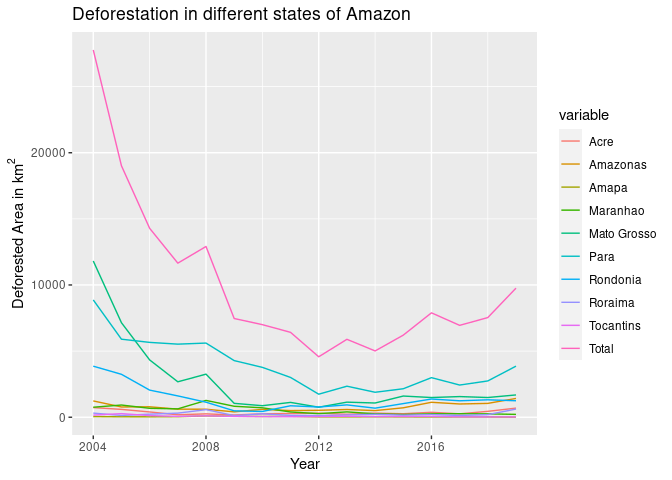
\includegraphics{Fire_files/figure-latex/unnamed-chunk-5-1.pdf}

\begin{Shaded}
\begin{Highlighting}[]
\NormalTok{drought[drought }\SpecialCharTok{==} \DecValTok{0}\NormalTok{] }\OtherTok{\textless{}{-}} \ConstantTok{NA}
\FunctionTok{tm\_shape}\NormalTok{(World,}\AttributeTok{bbox =}\NormalTok{ stars}\SpecialCharTok{::}\FunctionTok{st\_as\_stars}\NormalTok{(drought))}\SpecialCharTok{+}\FunctionTok{tm\_polygons}\NormalTok{() }\SpecialCharTok{+}
  \FunctionTok{tm\_shape}\NormalTok{(drought)}\SpecialCharTok{+}\FunctionTok{tm\_raster}\NormalTok{(}\AttributeTok{n=}\DecValTok{4}\NormalTok{)}
\end{Highlighting}
\end{Shaded}

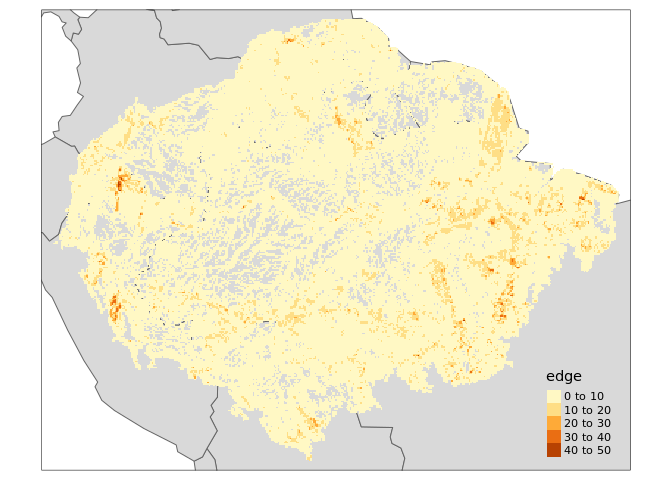
\includegraphics{Fire_files/figure-latex/unnamed-chunk-6-1.pdf}

\begin{Shaded}
\begin{Highlighting}[]
\NormalTok{edge[edge }\SpecialCharTok{==} \DecValTok{0}\NormalTok{] }\OtherTok{\textless{}{-}} \ConstantTok{NA}
\FunctionTok{tm\_shape}\NormalTok{(World,}\AttributeTok{bbox =}\NormalTok{ stars}\SpecialCharTok{::}\FunctionTok{st\_as\_stars}\NormalTok{(edge))}\SpecialCharTok{+}\FunctionTok{tm\_polygons}\NormalTok{() }\SpecialCharTok{+}
  \FunctionTok{tm\_shape}\NormalTok{(edge)}\SpecialCharTok{+}\FunctionTok{tm\_raster}\NormalTok{(}\AttributeTok{n=}\DecValTok{4}\NormalTok{)}
\end{Highlighting}
\end{Shaded}

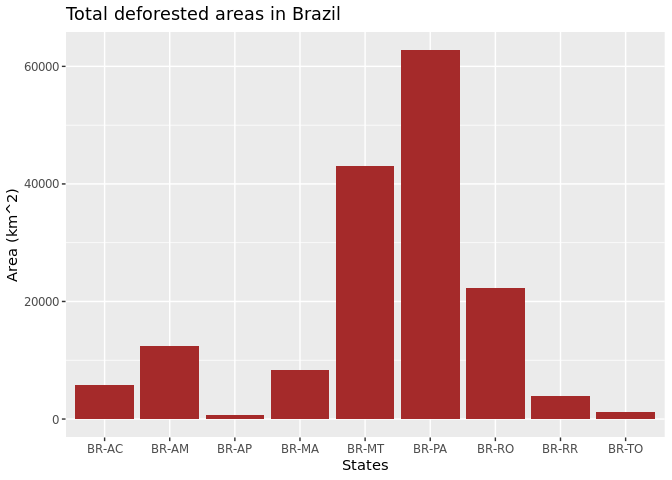
\includegraphics{Fire_files/figure-latex/unnamed-chunk-7-1.pdf}

\begin{Shaded}
\begin{Highlighting}[]
\NormalTok{logging[logging }\SpecialCharTok{==} \DecValTok{0}\NormalTok{] }\OtherTok{\textless{}{-}} \ConstantTok{NA}
\FunctionTok{tm\_shape}\NormalTok{(World,}\AttributeTok{bbox =}\NormalTok{ stars}\SpecialCharTok{::}\FunctionTok{st\_as\_stars}\NormalTok{(logging))}\SpecialCharTok{+}\FunctionTok{tm\_polygons}\NormalTok{() }\SpecialCharTok{+}
  \FunctionTok{tm\_shape}\NormalTok{(logging)}\SpecialCharTok{+}\FunctionTok{tm\_raster}\NormalTok{(}\AttributeTok{n=}\DecValTok{4}\NormalTok{)}
\end{Highlighting}
\end{Shaded}

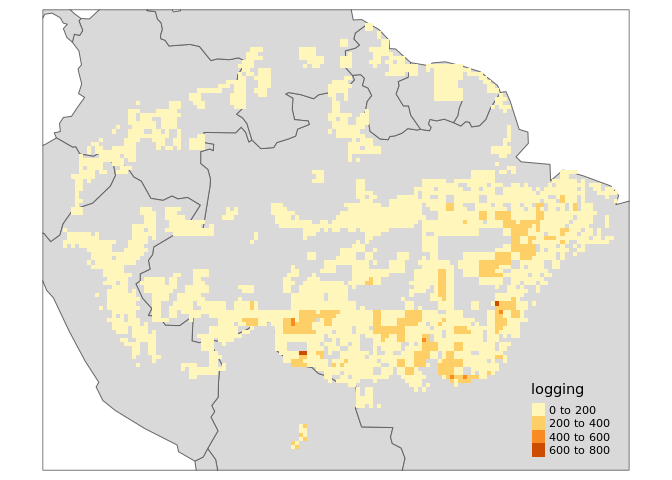
\includegraphics{Fire_files/figure-latex/unnamed-chunk-8-1.pdf}

\end{document}
